\documentclass{article}
\usepackage{blindtext}
\usepackage[a4paper, total={6in, 9.4in}]{geometry}
\usepackage{indentfirst}
\usepackage{wrapfig}
\usepackage{graphicx}
\usepackage{mathtext}
\usepackage{amsmath}
\usepackage{siunitx} % Required for alignment
\usepackage{subfigure}
\usepackage{multirow}
\usepackage{rotating}
\usepackage{afterpage}
\usepackage[T1,T2A]{fontenc}
\usepackage[russian]{babel}
\usepackage{caption}
\usepackage[arrowdel]{physics}
\usepackage{booktabs}

\graphicspath{{pictures/}}

\title{\begin{center}Лабораторная работа №4.2.1\end{center}
Кольца Ньютона}
\author{Гёлецян А.Г.}
\date{\today}

\begin{document}

\pagenumbering{gobble}
\maketitle
\newpage
\pagenumbering{arabic}

\textbf{Цель работы:} познакомиться с явлением интерференции в тонких пленках
на примере колец Ньютона и с методикой интерференционных измерений кривизны
стеклянной поверхности.

\section{Теоретическая часть}
\begin{wrapfigure}{l}{0.35\linewidth} 
    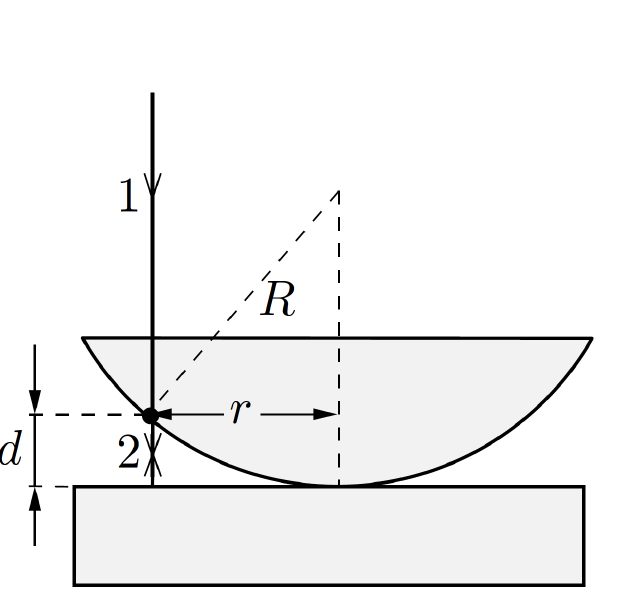
\includegraphics[width=\linewidth]{lens.png}
    \caption{Экспериментальная установка}\label{fig:lens}
\end{wrapfigure}

Этот классический опыт используется для определения радиуса кривизны сферических
поверхностей линз. В этом опыте наблюдается интерференция волн, отражённых от границ
тонкой воздушной прослойки, образованной сферической поверхностью линзы и плоской
стеклянной пластиной. При нормальном падении света (рис.~\ref{fig:lens})
интерференционные полосы локализованы на сферической поверхности и являются
полосами равной толщины.
	
Геометрическая разность хода между интерферирующими лучами равна удвоенной толщине
воздушного зазора $ 2d $ в данном месте. Для точки на сферической поверхности,
находящейся на расстоянии $ r $ от оси системы, имеем
$ r^2 = R^2 - {(R - d)}^2 = 2Rd - d^2 $, где $ R $ --- радиус кривизны сферической
поверхности (рис.~\ref{fig:lens}).
	
	При $R\gg d$ получим $d = r^2/2R$. С учётом изменения фазы на $\pi$ при отражении волны от оптически более плотной среды (на границе воздух-стекло) получим \textbf{оптическую разность хода интерферирующих лучей}:
	
\begin{equation}\label{r_m}
    \Delta = \dfrac{\lambda}{2} + 2d = \dfrac{r^2}{R} + \dfrac{\lambda}{2}
\end{equation}
	
Из условия интерференционного минимума
$ \Delta = \dfrac{(2m +1)\lambda}{2}, \; m =0, 1, 2.. $ получим радиусы темных
колец $ r_m $, а из аналогичного условия максимума $ \Delta = m \lambda $
радиусы светлых $r_m'$:
	
\begin{equation}\label{r_m'}
    r_m = \sqrt{m \lambda R}, \qquad r_m' = \sqrt{\dfrac{(2m-1) \lambda R}{2}}
\end{equation}

\section{Ход работы}
\subsection{Калибровка шкалы микроскопа}
На рис. \ref{fig:calibration} видно, что 6 делениям микроскопа соотвествуют 5.9 делений
откалиброванной шкалы. Следовательно, 1 деление микроскопа $\approx$ 98.3 мкм.

\begin{figure}[h]
    \center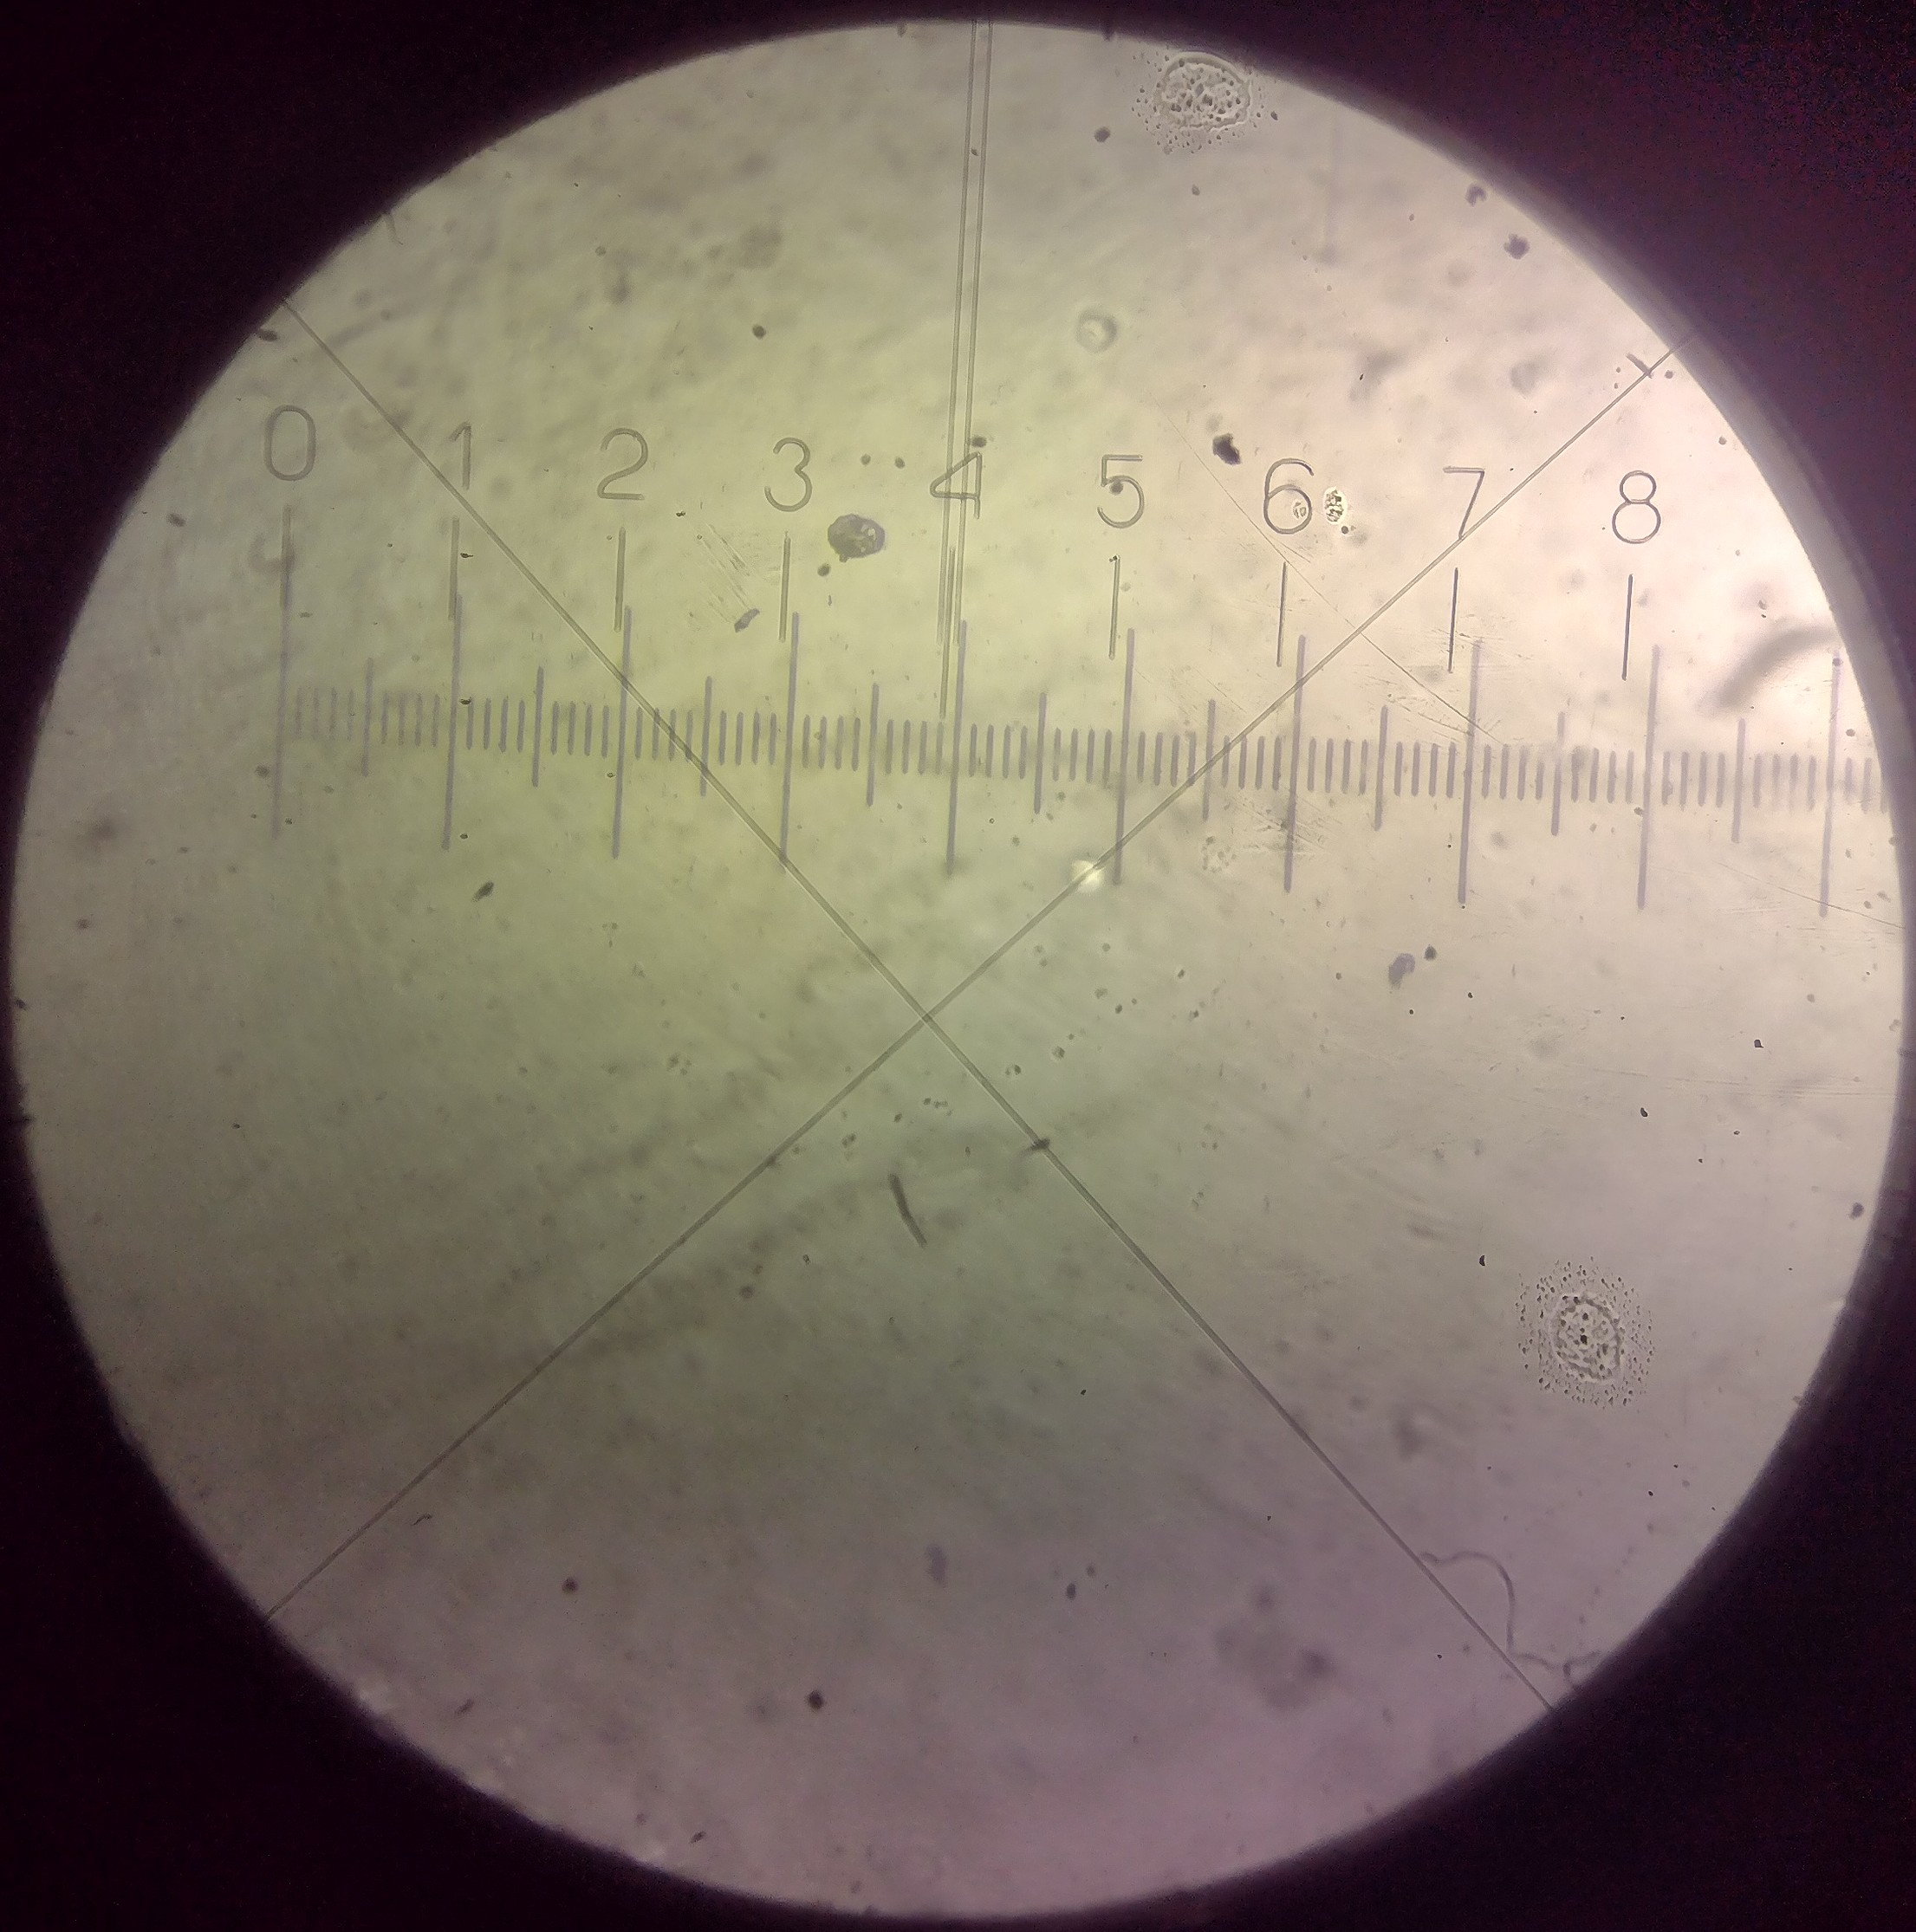
\includegraphics[width = 0.3\linewidth]{calibration.jpg}
    \caption{Калибровка шкалы микроскопа}\label{fig:calibration}
\end{figure}

\subsection{Измерение радиуса кривизны линзы}


\begin{table}[h!]
\vspace{5pt}
\begin{center}\subtable{
    \begin{tabular}{rr}
    \toprule
     m &  $r_m$, мкм \\
    \midrule
     1 &  87.5 \\
     2 & 120.9 \\
     3 & 148.9 \\
     4 & 171.5 \\
     5 & 190.7 \\
     6 & 209.4 \\
     7 & 225.6 \\
     8 & 240.8 \\
     9 & 255.6 \\
    10 & 269.8 \\
    11 & 281.1 \\
    \bottomrule
    \end{tabular}
}\subtable{
    \begin{tabular}{rr}
    \toprule
     m &  $r_m'$, мкм \\
    \midrule
     1 &  62.4 \\
     2 & 107.6 \\
     3 & 135.7 \\
     4 & 160.2 \\
     5 & 180.9 \\
     6 & 199.5 \\
     7 & 216.8 \\
     8 & 233.5 \\
     9 & 247.7 \\
    10 & 262.0 \\
    11 & 275.7 \\
    \bottomrule
    \end{tabular}
}
    \caption{Радиусы темных ($r_m$) и светлых ($r_m'$) колец}\label{ring_radii}
\end{center}
\end{table}

\begin{figure}[h]
    \center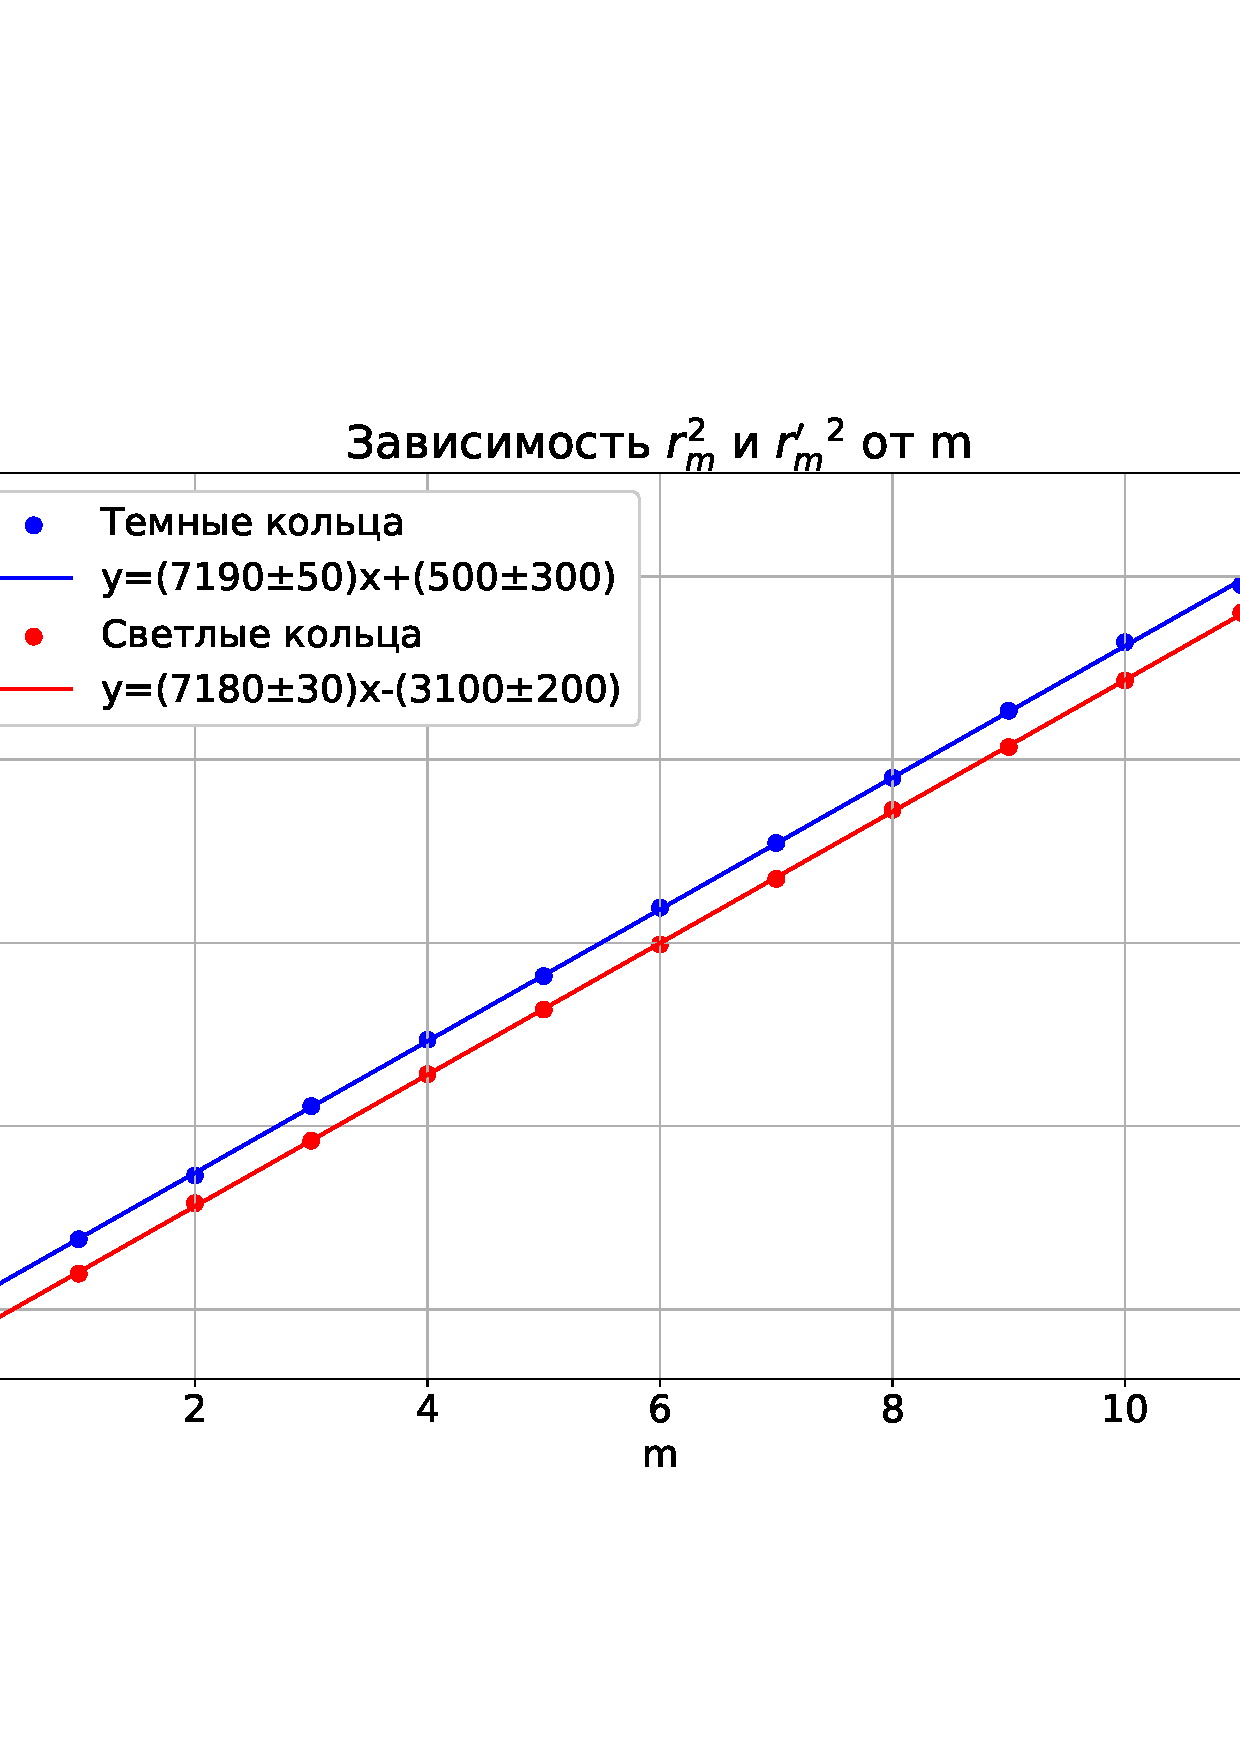
\includegraphics[width = 0.8\linewidth]{linearized}
    \caption{Линеаризованные графики радиусов колец}\label{fig:linearized}
\end{figure}

Как видим, наклоны прямых практически равны, поэтому для простоты возмьем среднее
значение $(7185 \pm 40)$ мкм$^2$. Согласно формулам (1) и (2) наклоны прямых равны
$\lambda \cdot R$. Длины волн компонент желтого дуплета ртутной лампы $577 \pm 10$ нм.
Отсюда можем найти радиус кризны линзы

\begin{equation}
    R = (1.25 \pm 0.02) \text{ см}
\end{equation}

\newpage

\begin{figure}[h]
    \center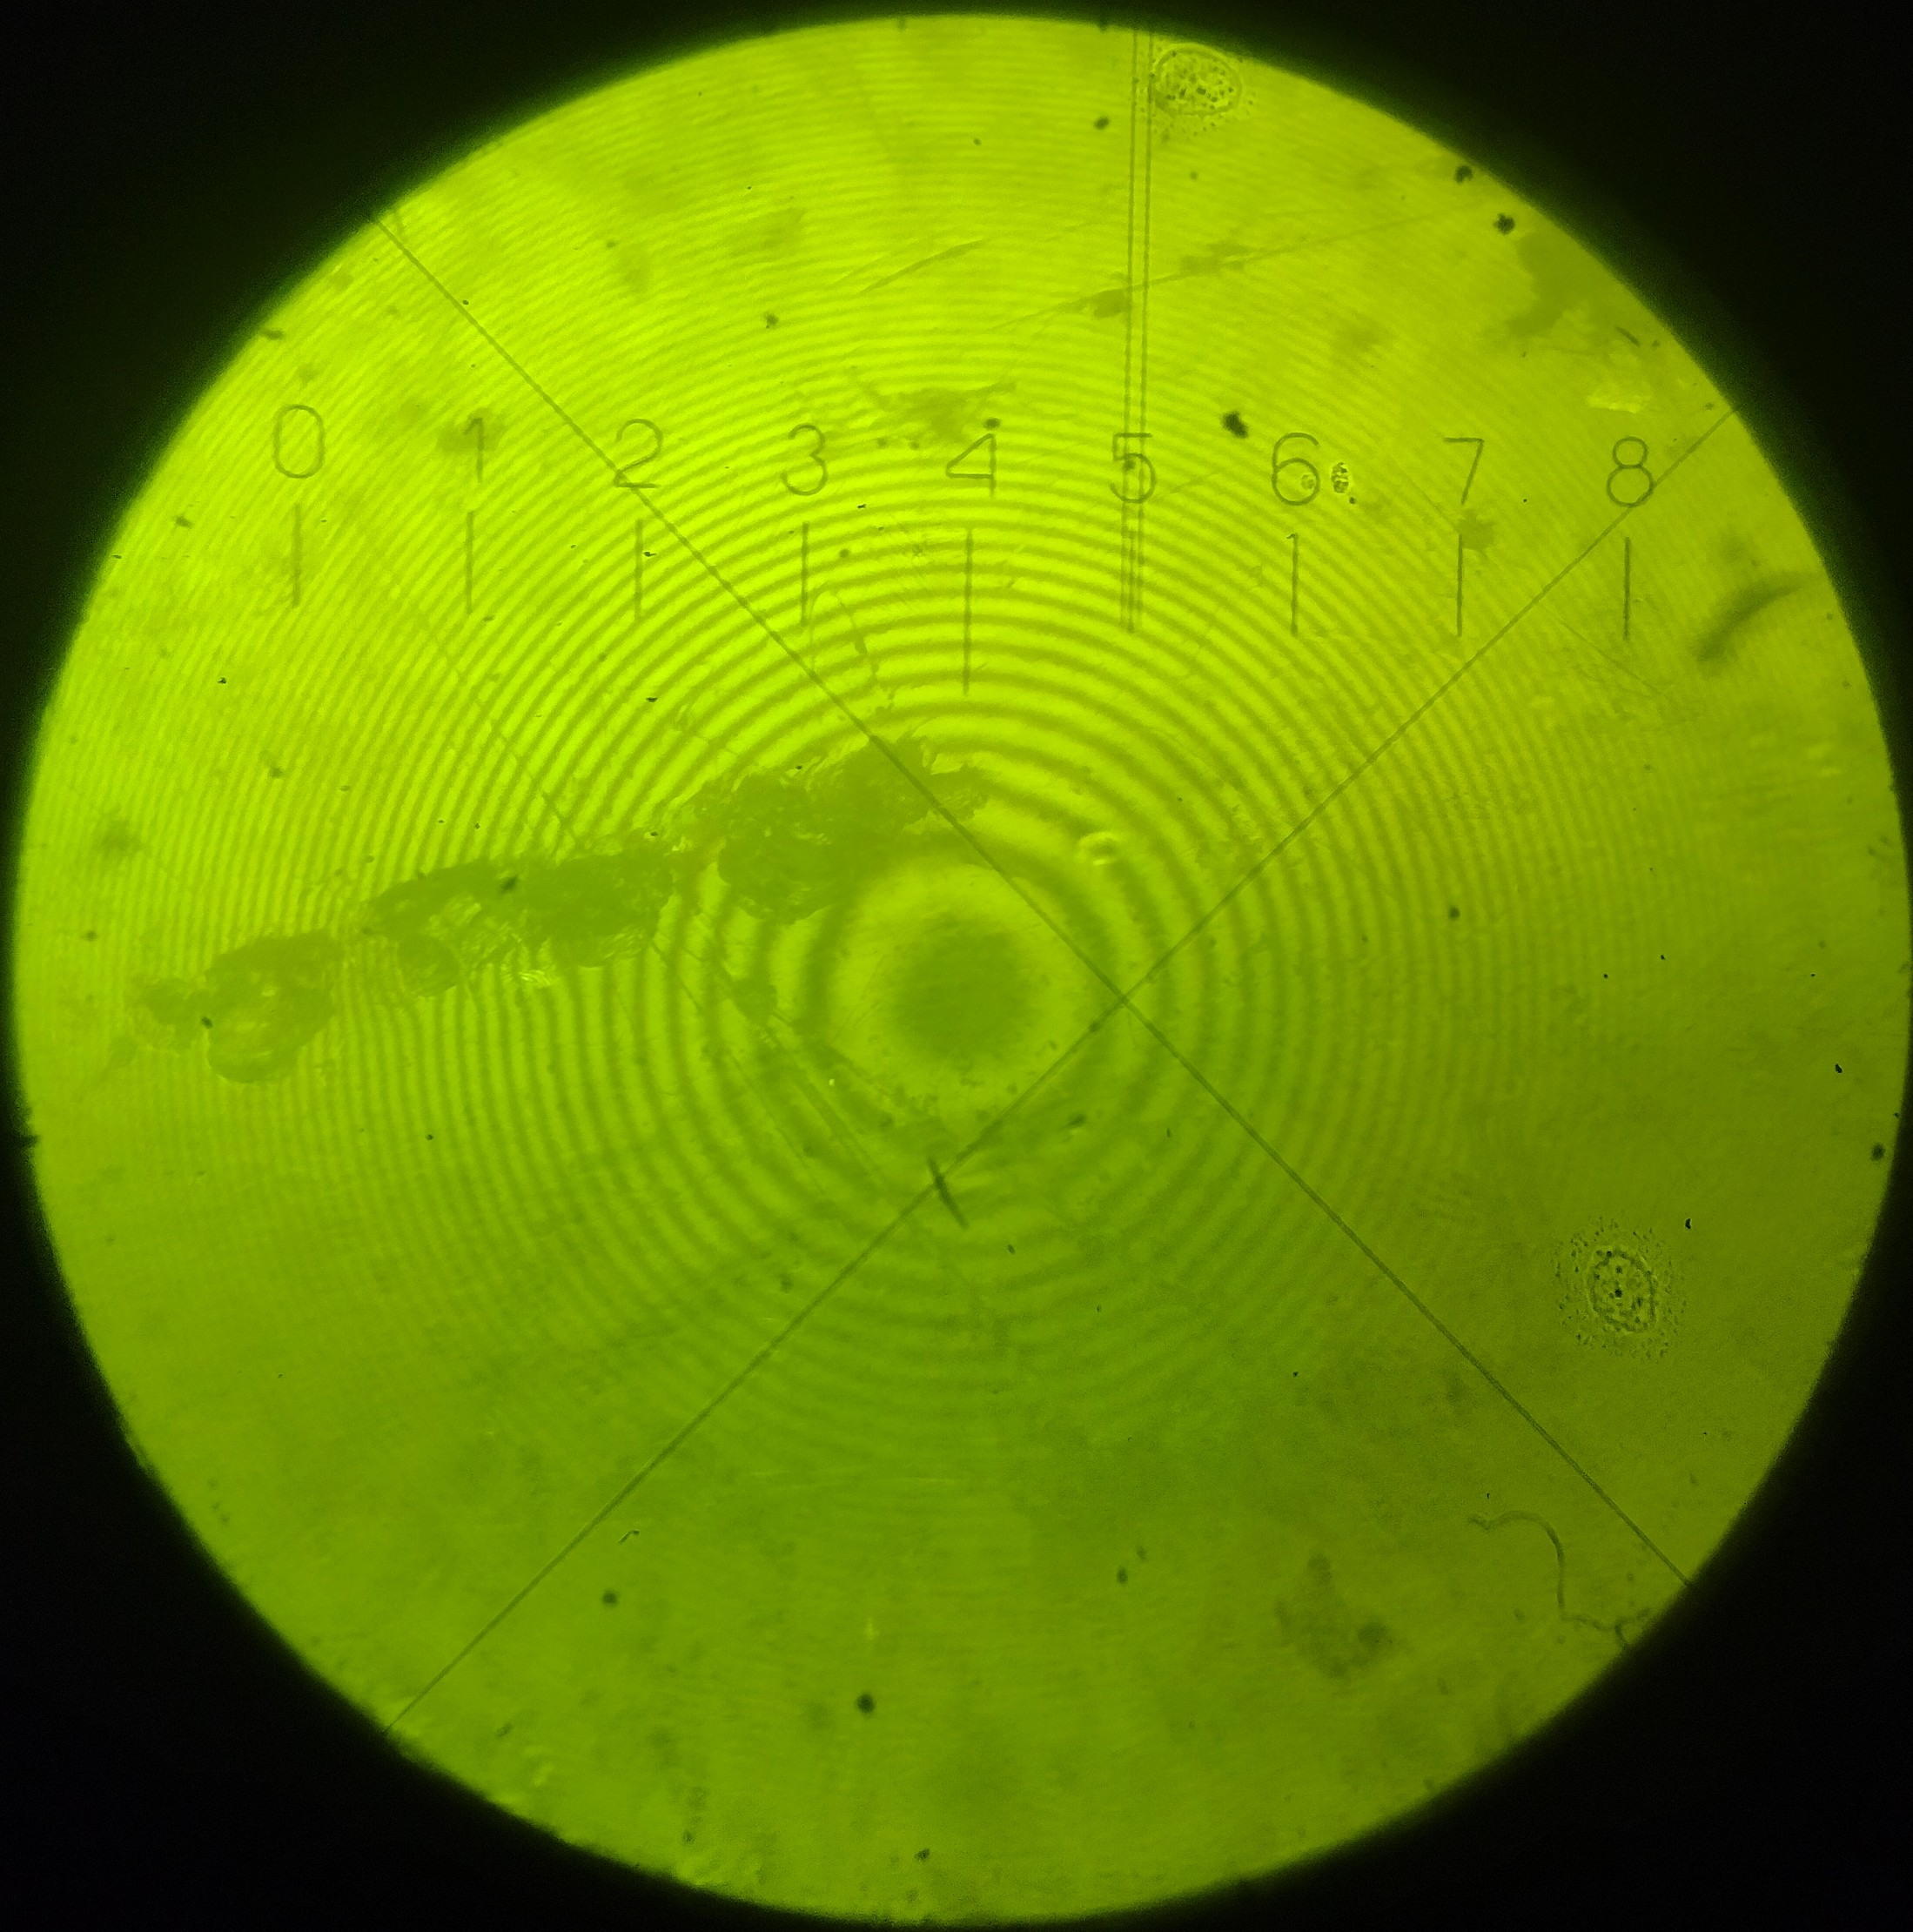
\includegraphics[width = 0.6\linewidth]{rings.jpg}
    \caption{Кольца Ньютона}\label{fig:rings}
\end{figure}

\subsection{Биения}
При пропускнии света с двумя компонентами монохроматичности возникают биения вследствии
наложения двух систем колец. Когда максимумы одной системы ложатся на минимумы другой
системы, четкость картинки теряется. Период границ четкости (в кольцах) приблизительно
равен $\Delta m = \lambda / {\Delta \lambda}$. Визуальными измерениями получили период
границ четкости в 18 полос. $\lambda \approx 577$ нм $\implies$
$\Delta \lambda \approx 32$ нм. Из данных про спектр ртутной лампы имеем
$\lambda_1=577$ нм, $\lambda_2=546$ нм, $\Delta \lambda_{табл} = 33$ нм.

\section{Выводы}
Успешно пронаблюдали кольца Ньютона, которые появляются вследствие многолучевой
интерференции в зазоре между линзой и черным стеклом. Радиусы светлых и темных колец с
хорошей точностью описываются теоретической формулой.

Пронаблюдали биения интерференционной картины вследствии немонохроматичности света.
Оценка разности длин волн спектральных компонент в световой смеси достаточно близко
к табличным значениям, однако это ни о чем не говорит, потому что оценка строится
на не совсем точных принципах, а погрешность измерения границ четкости сильно большая
из за незоркого зрения наблюателя.


\end{document}
